\documentclass[10pt,a4paper,1.5lines]{article}
\usepackage[utf8]{inputenc}
\usepackage{indentfirst}        % Indentación de todos los párrafos
% \usepackage{amsmath}
% \usepackage{amsfonts}
% \usepackage{amssymb}
\usepackage{graphicx}           % Gráficos, imágenes
\usepackage{subfig}
\usepackage{setspace}           % interlineado
%\usepackage{flushend}           % nivelar columnas
\usepackage[]{hyperref}         % Hiperenlaces
%\usepackage{pdflscape}          % paginas apaisadas
\usepackage{colortbl}           % Tablicas con colores
\usepackage[left=2cm,right=2cm,top=2cm,bottom=2cm]{geometry}
\usepackage[printonlyused,withpage]{acronym}        % acrónimos
\usepackage[table,cmyk,usenames,dvipsnames,pdftex]{xcolor}

\onehalfspacing

\newcommand{\todo}[1][ToDo]{
  \textcolor{WildStrawberry}{
    \Large{\textbf{#1}}
  }
}

\author{Ignacio D\'iez}
\title{Analysis of Volleyball Results}

\setlength{\columnsep}{2em}

\begin{document}

\maketitle

\begin{abstract}
This paper presents a comprehensive analysis of the results from the \ac{NVL} under Volleyball England over the past two decades, encompassing twenty full seasons of competitive play. The study is structured in two main parts. The first part explores long-term historical trends, focusing on team performance, competitive balance, and league dynamics from a macro perspective. \todo[It identifies dominant clubs, performance fluctuations], and statistical patterns that have emerged across seasons, supported by a series of charts and visual data representations. The second part narrows its scope to the current 2024/2025 season, offering a more granular and localized analysis. This includes club-specific insights, individual team and referee metrics, and an evaluation of referee assignments. By combining longitudinal data with current-season specifics, this study aims to provide both a retrospective understanding and a real-time snapshot of the state of volleyball in England, contributing valuable insight to players, coaches, analysts, and enthusiasts of the sport.\end{abstract}

\section{Methodology}
The \ac{VE} website hosts the results for \ac{NVL},  and Cup\&Shield games played since the 2005/06 season. I thought it would be interesting to download and analyse that data, and see what information can be inferred from it.

I created a script to scrape\footnote{Web scraping refers to the act of using software to automate the download of information from a web page, using a bot or a web crawler, and storing it for later retrieval or analysis. See \url{https://en.wikipedia.org/wiki/Web_scraping} for more information.} the website and download all the individual results, from each season, and for each category and division. The script downloaded the raw \ac{HTML} page and stored it for later processing.

Then, I wrote a Python parser to read all those \ac{HTML} files and extract the necessary information hidden inside: date, names of the teams, category, division, score, points, venue, name of referee$\ldots$ Unfortunately, the names of the referees are only available since the 2023/2024 season. However, the rest of the data is all there.

All the information was converted into sensible data structures and stored into \ac{CSV} files, so that it could be easily accessed and processed. After that, it was a matter of thinking what kind of visualization (charts) and information would be interesting to obtain.

In total, there are 8430 games recorded, spanning over 20 years, 2 competitions (\ac{NVL} and Cup\&Shield), 2 categories (Men and Women) and 5 divisions (Superleague --includes the former Super8--, Div1, Div2, Div3 and a special division "Playoffs"); also, more than \todo[50] teams and 350 referees were also listed.

\section{Errors and Discarded data}
While creating the chars and processing the data, I noticed some errors in the input; impossible results that were clearly mistakes (e.g. a set that had 256 points, or less that 25 for both teams but was not the 5\textsuperscript{th}). Some of those errors are obvious and were fixed when possible. Table \ref{table:error} (on page \pageref{table:error}) contains a list of all the games that were discarded (i.e. excluded from the calculations) due to incorrect results. 

%\begin{landscape}
	\begin{table}
		\centering
		\begin{tabular}{|l|l|l|c|ccccc|}
			\hline
			\rowcolor{Goldenrod}%
			\textbf{Date} & \textbf{Division} & \textbf{Teams} & \textbf{Sets} & \multicolumn{5}{c|}{\textbf{Points}}\\	\hline
			2008-01-06 & Shield Women & Sheffield & 3 & 256 & 25 & 25 & - & - \\
			&      & Dartford Crossers & 0 & 0   & 0  & 0  & - & - \\
			\hline
			2015-04-26 & Superleague Men & Northumbria University & 1 & 15 & 0 & 0 & - & - \\
			&                 & Sheffield              & 0 & 12 & 0 & 0 & - & - \\
			\hline
			2017-04-23 & Superleague Women & Durham Palatinates & 1 & 15 & 0 & 0 & - & - \\
			&        & Team SideOut Polonia (London) & 0 & 9  & 0 & 0 & - & - \\
			\hline
			2017-04-23 & Superleague Men & Northumbria University & 0 & 12 & 0 & 0 & - & - \\
			&                 & Sheffield              & 1 & 15 & 0 & 0 & - & - \\
			\hline
			2018-04-22 & Superleague Women & Durham Palatinates & 0 & 15 & 0 & 0 & - & - \\
			&        & Team SideOut Polonia (London) & 1 & 5  & 0 & 0 & - & - \\
			\hline
			2018-05-06 & Superleague Women & Northumbria University & 0 & 13 & 0 & 0 & - & - \\
			&                   & Durham Palatinates     & 1 & 15 & 0 & 0 & - & - \\
			\hline
			2022-09-25 & Cup Women & Ashcombe Dorking & 3 & 25 & 25 & 25 & - & - \\
			&           & UK Armed Forces  & 2 & 0  & 0  & 0  & - & - \\
			\hline
			2023-04-01 & Division 1 Men & London Aces & ? & 0 & 0 & 0 & - & - \\
			&        & Manchester Marvels  & ? & 0 & 0 & 0 & - & - \\
			\hline
			2023-04-09 & Division 2 Women & Urbond VC Portsmouth & ? & - & - & - & - & - \\
			&                  & Essex Trinity        & ? & - & - & - & - & - \\
			\hline
			2023-08-02 & Cup Men & Wolverhampton & ? & 0 & 0 & 0 & 0 & 0 \\
			&         & Brighton      & ? & 0 & 0 & 0 & 0 & 0 \\
			\hline
			2023-09-09 & Cup Men & London Wildcats & 3 & - & - & - & - & - \\
			&         & London Bears    & 2 & - & - & - & - & - \\
			\hline
			2023-09-10 & Cup Women & Reading Aces & 1 & - & - & - & - & - \\
			&           & London Bears & 3 & - & - & - & - & - \\
			\hline
			2023-09-23 & Cup Men & Team SideOut (London) & 3 & - & - & - & - & - \\
			&         & Army                  & 0 & - & - & - & - & - \\
			\hline
			2023-11-11 & Shield Men & London Bears & 3 & - & - & - & - & - \\
			&            & Men          & 1 & - & - & - & - & - \\
			\hline
			2023-12-02 & Shield Women & Waterloo Thunder Volleyball Club & ? & - & - & - & - & - \\
			&              & Onyx London                      & ? & - & - & - & - & - \\
			\hline
		\end{tabular}
		\caption{List of wrong results}
		\label{table:error}
	\end{table}
%\end{landscape}


\section{Data Analysis}
\todo[review the intro]
This section presents a comprehensive examination of volleyball game results in England over the past two decades. By leveraging historical data from the last 20 seasons, we aim to uncover broad trends, patterns, and shifts in the sport’s competitive landscape. Through visualizations and statistical insights, we establish a long-term context that sets the foundation for understanding the evolution of teams, performance consistency, and competitive dynamics. In parallel, we take a closer look at the current season to spotlight more granular aspects, such as referee influence and club-specific characteristics, providing a richer, more nuanced understanding of the present-day game.

\subsection{Long-time data}
\label{sub:long-range}

\todo[review the intro]

This subsection investigates the full archive of match results spanning the last 20 seasons of English volleyball. The focus here is on identifying macro-level patterns, such as dominant teams over time, seasonal win-loss distributions, changes in competitive balance, and the evolution of game dynamics. A series of charts and graphs will support this analysis, offering visual representations of league trajectories, performance cycles, and notable statistical anomalies. By establishing a long-term view, this analysis sets the stage for comparisons with present-day developments.

\subsubsection{Points Distribution}
By plotting the number of total points in a game (i.e. the sum of all the points scored by both teams) we can get an idea of what an average game looks like.

Figure \ref{fig:point-histogram} shows the point distribution by sex. The men data is slightly shifted to the right, which indicates that men games tend to have more points in total. This could mean that the level among men teams is more homogeneous than in women teams. However, the difference is not significative.

\begin{figure}
	\centering
	\subfloat[Points by category]{{
			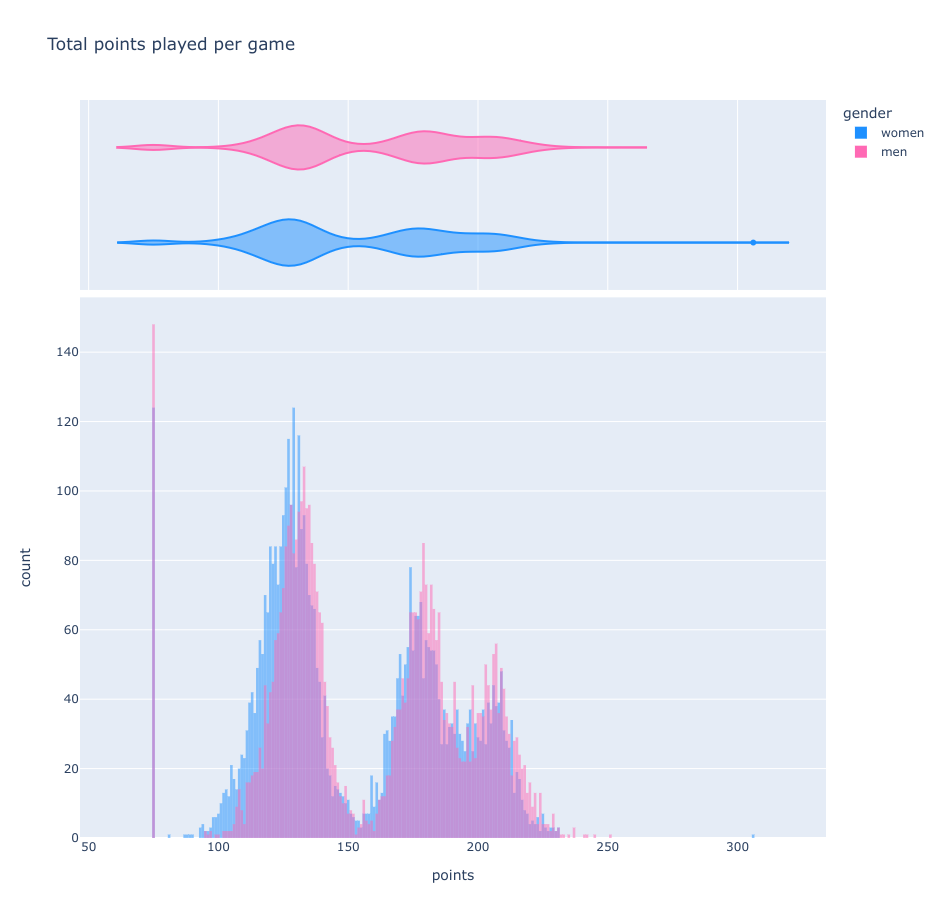
\includegraphics[width=.4\linewidth]{points-histogram-sex.png}
	}}
	\qquad
	\subfloat[Points by number of sets]{{
			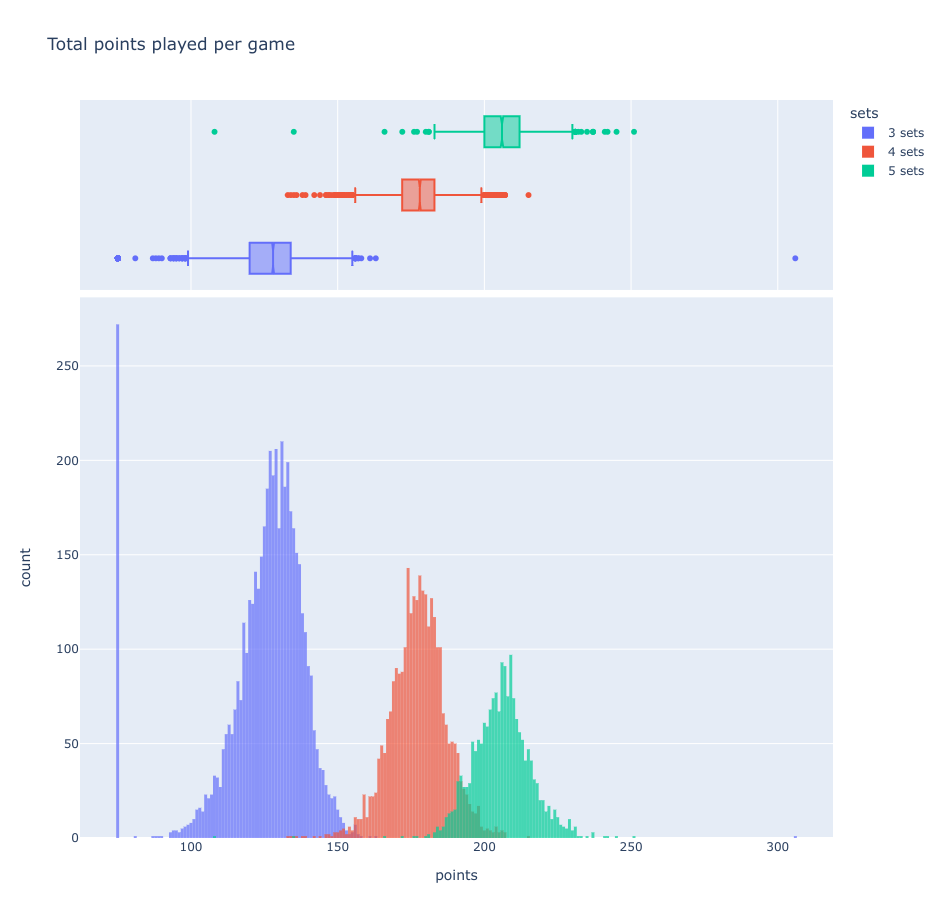
\includegraphics[width=.4\linewidth]{points-histogram-sets.png}
	}}
	
	\caption{Histograms showing the distribution of the total match points}
	\label{fig:point-histogram}
\end{figure}

The lonely column on the far left are the games with a total point sum of 75. These can only happen if the result is 25-0 25-0 25-0, which indicates a forfeit. The chart shows that men tend to forfeit around 25\% more than women, with 146 games forfeited by men, versus 116 by women.

The 3 peaks that can be observed in the histogram correlate to the number of sets. This can be better observed in figure \ref{fig:point-histogram}. In blue are the games that were just 3 sets long. This includes the forfeits, prominently displayed on the left again. As expected, the number of 3-set games is greater than the number of 4-set games, which is in turn greater than the number of 5-set games.

We can also observe that the overlap in the number of points between 3 and 4 set games is much smaller than the overlap between 4 and 5 set games. This is of course due to the 5\textsuperscript{th} set being capped at 15 points.

The games seem to follow a normal distribution, meaning that extreme results --such as 25-3, for example-- are quite rare; and on average, teams are evenly matched.

\subsubsection{Game Results}
As stated earlier, 3-set games are the most common by far, accounting for ~52\% of the results. Games to 4 sets add up to ~30\% of the outcomes, while only ~18\% of games reach the tie-breaker.
Of those results, most of the times a home victory is expected 55\% of times, indicating that a familiar environment does actually cause some effect --albeit only marginally--. Breaking down these findings by division, we can see that the higher the division, the more important it seems to be to play "at home", as shown in figure \ref{fig:home-victories-per-division}. I was really not expecting this, since I assumed that higher level players would be more\ldots professional, for lack of a better word, and they would be impervious to environment changes.

Some of these games are played in neutral ground (e.g. the Cup finals), which might skew the results a bit. However, the amount of these occurrences is too small to be significative, so no further refinement was made.

\begin{figure}
	\centering
	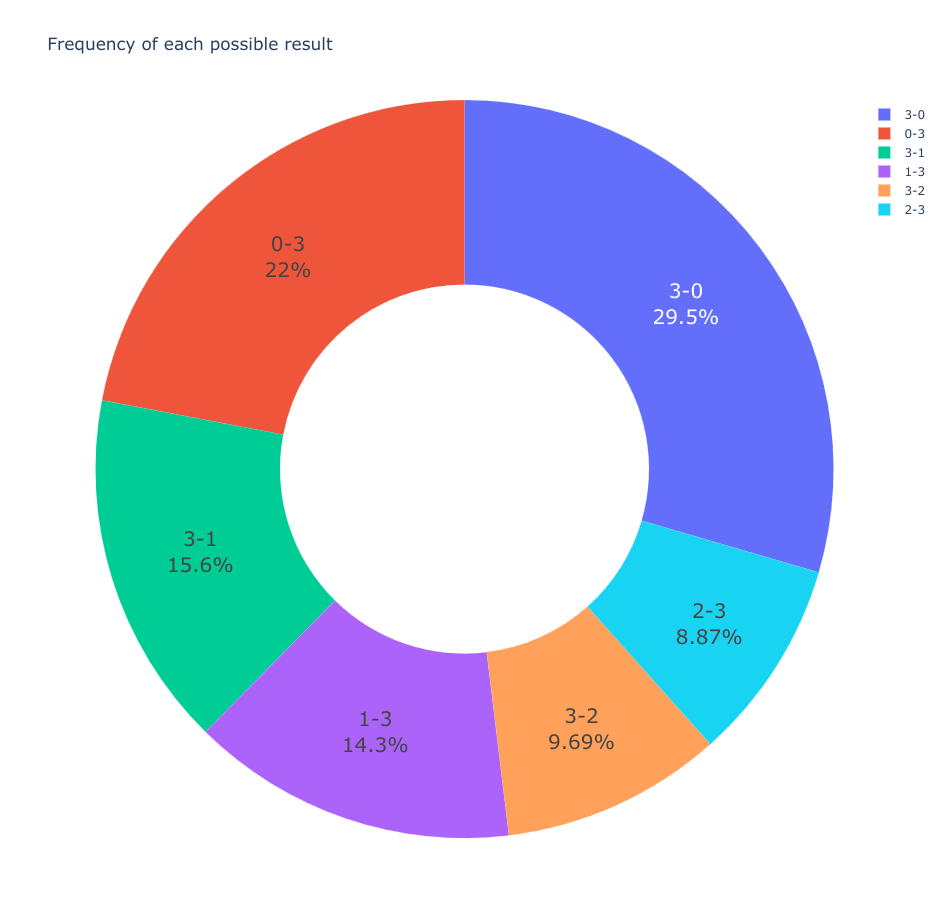
\includegraphics[width=.7\linewidth]{results-pie-chart.png}
	\caption{Frequency of each possible result}
	\label{fig:results-pie-chart}
\end{figure}

\begin{figure}
	\centering
	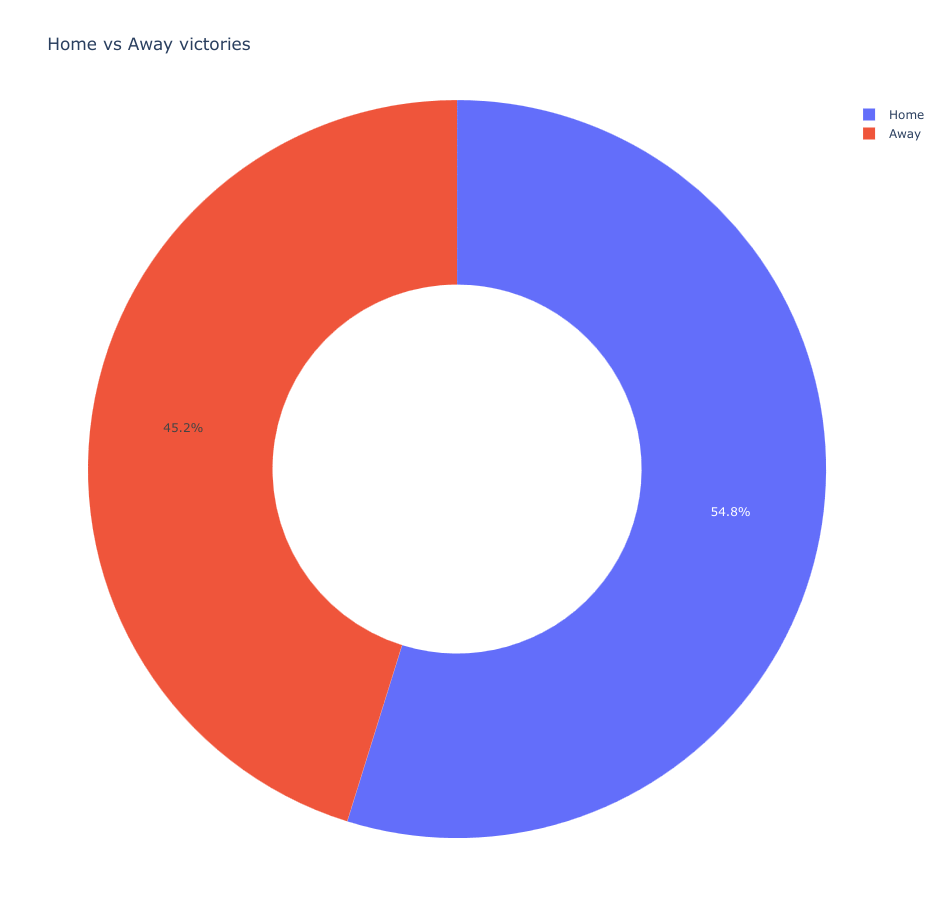
\includegraphics[width=.7\linewidth]{home-away-victories.png}
	\caption{Number of home vs away victories}
	\label{fig:home-away-victories}
\end{figure}

\begin{figure}
	\centering
	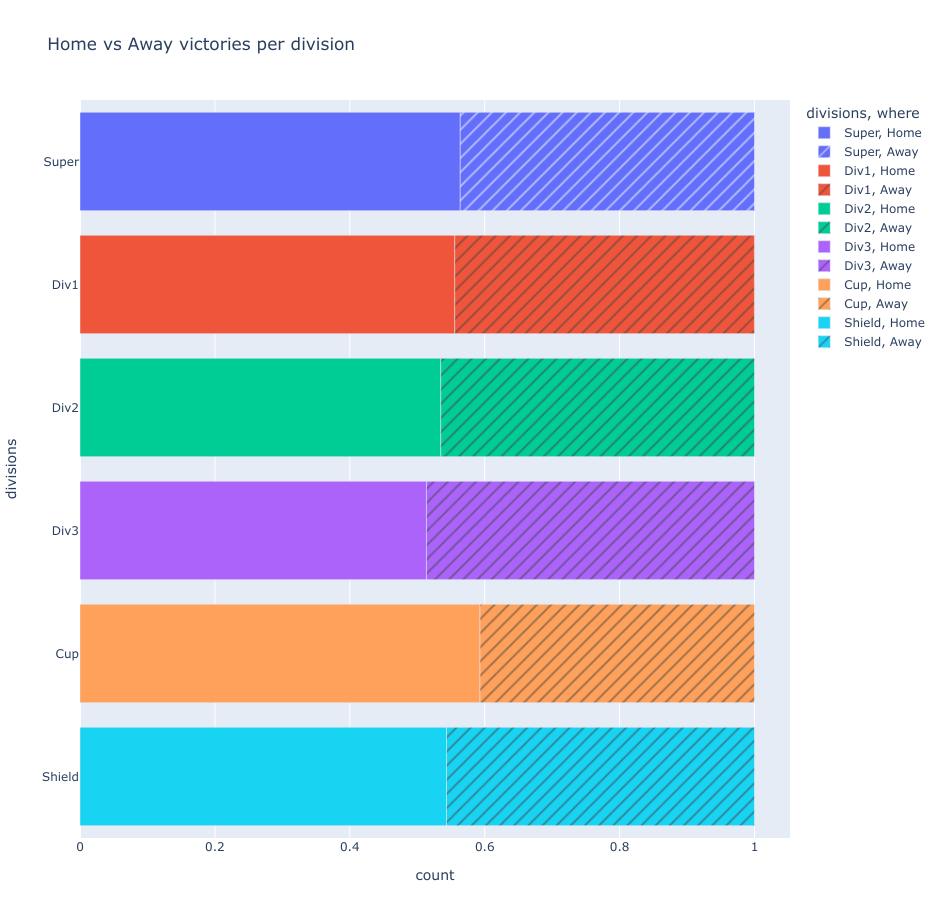
\includegraphics[width=.7\linewidth]{home-victories-per-division.png}
	\caption{Percentage of home victories, split by division}
	\label{fig:home-victories-per-division}
\end{figure}


\subsubsection{Evolution}
\ac{VE} has clearly been working to promote, develop and grow the sport in England, and the following charts are proof of it. Figure \ref{fig:games-per-year} plots the number of games each season, showing a massive increase since 183 games in 2005 to +1200 in 2025. That means a 7-fold increment. Particularly noticeable is the effect of COVID lockdown: there were no games in the 2020/2021 season, and the 2021/2022 season had to be cut short early, due to additional lockdown measures.

\begin{figure}
	\centering
	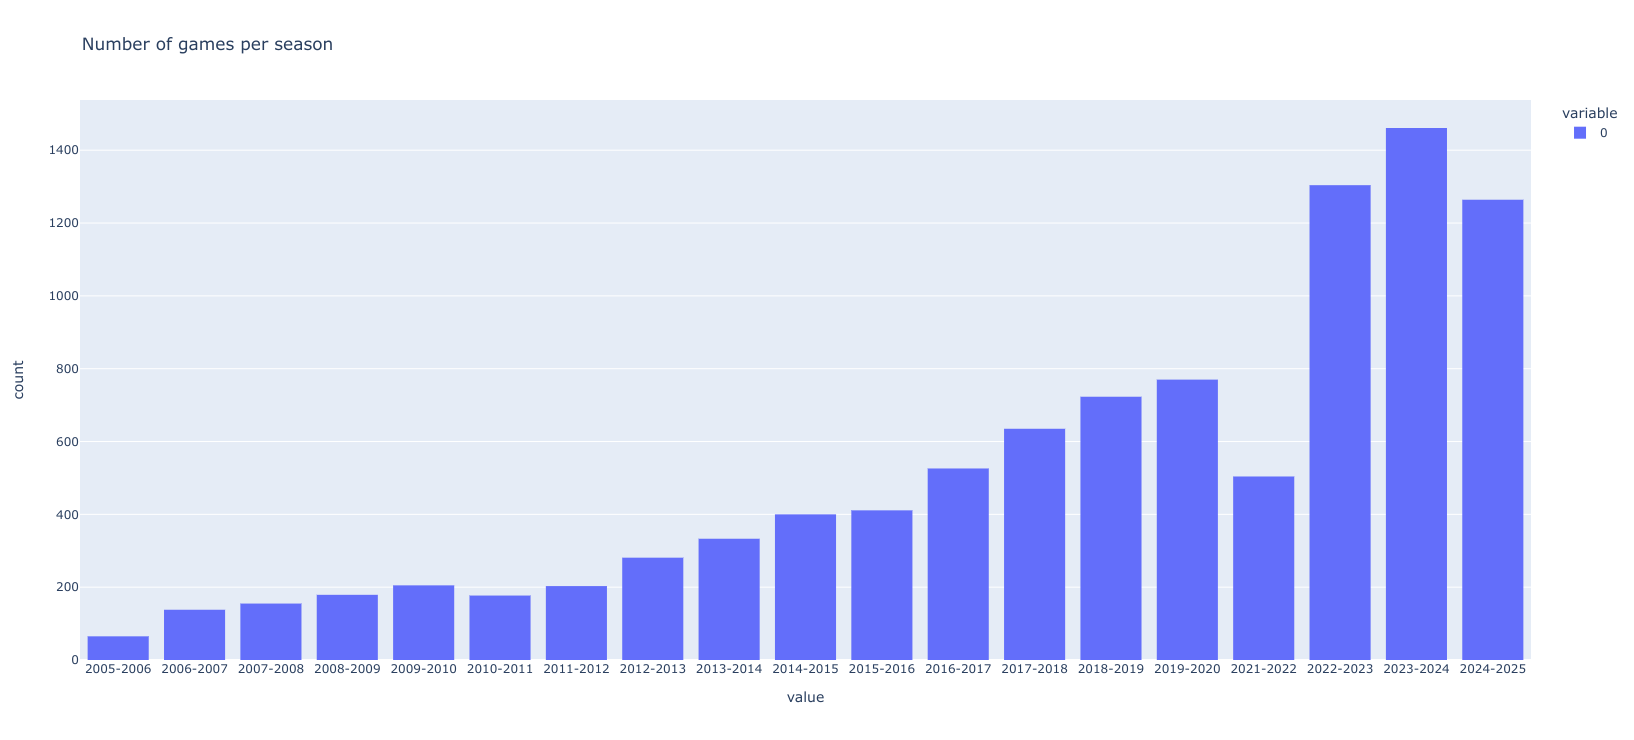
\includegraphics[width=0.7\linewidth]{games-per-year.png}
	\caption{Total number of games each season}
	\label{fig:games-per-year}
\end{figure}

If we split by division, shown in figure \ref{fig:games-per-year-by-division}, we can see the start of the Superleague (Super8) back in 2010. More importantly, we can see that the increase in the number of games has come mainly from a corresponding increase in Division 2 and specially Division 3, particularly since 2022.

\begin{figure}
	\centering
	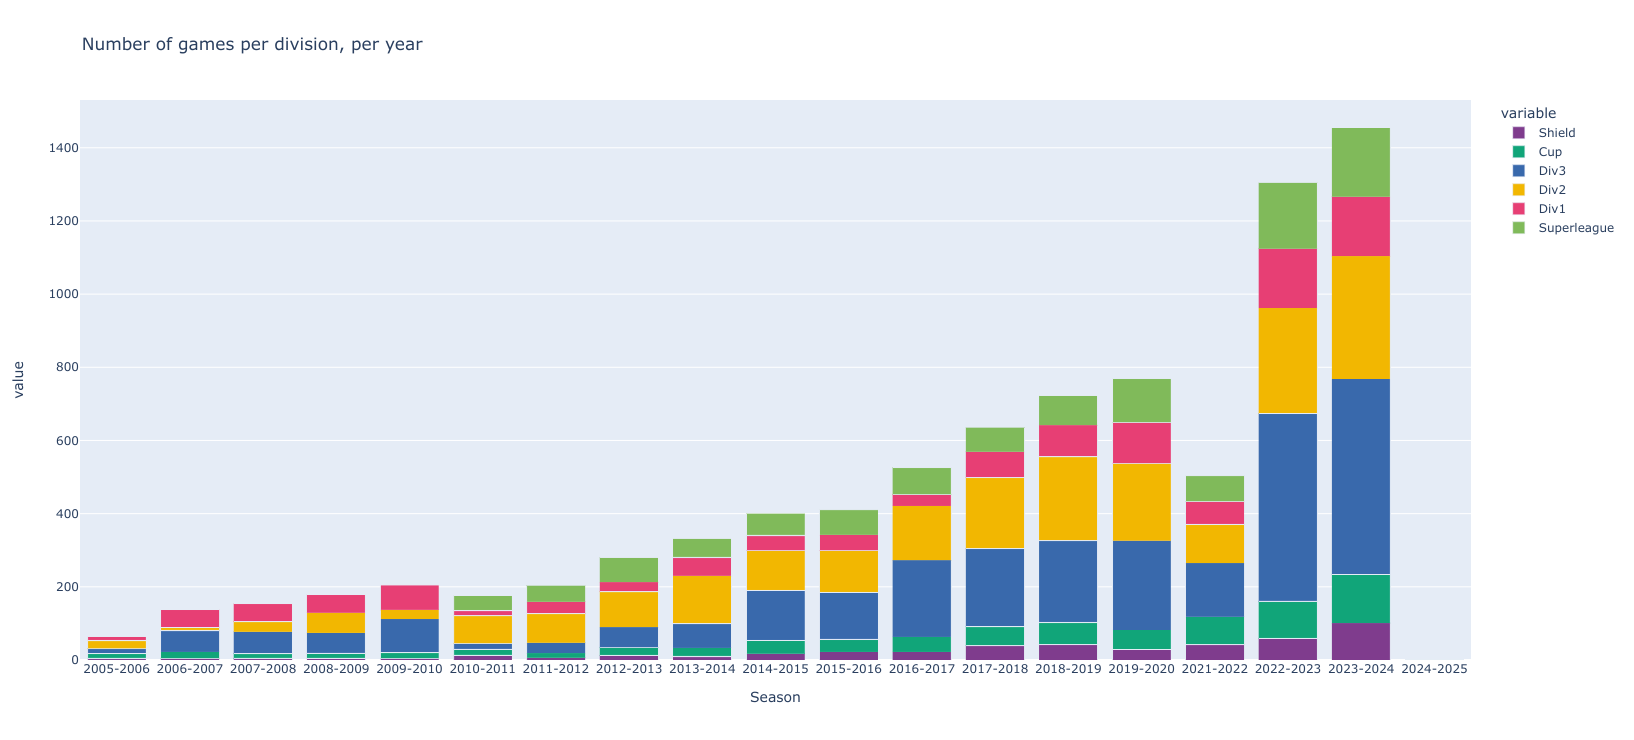
\includegraphics[width=0.7\linewidth]{games-per-year-by-division.png}
	\caption{Total number of games each season, split by division}
	\label{fig:games-per-year-by-division}
\end{figure}

One would expect these increments to be caused by a similar increase in the number of teams. However, figure \ref{fig:teams-per-year} shows that te biggest increments have happened in the Cup and Shield competitions, specially in the last couple of seasons.

\begin{figure}
	\centering
	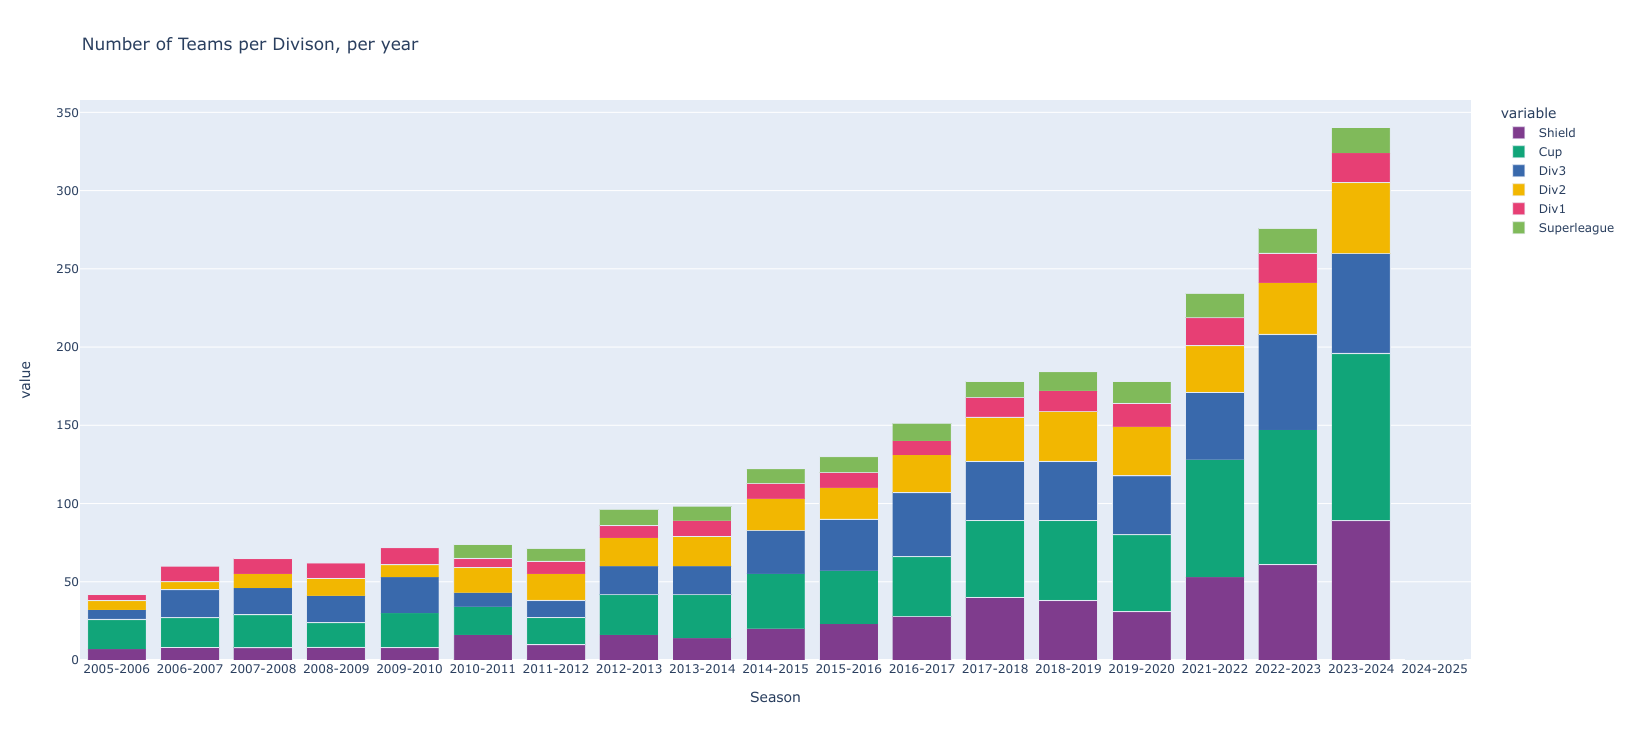
\includegraphics[width=0.7\linewidth]{teams-per-year.png}
	\caption{Number of teams competing in each division every season}
	\label{fig:teams-per-year}
\end{figure}


\subsection{Detailed study: 24/25 Season}
\label{sub:short-range}

\todo[review intro]

Shifting from a historical perspective to a more focused and immediate lens, this subsection explores detailed data from the ongoing volleyball season. Emphasis is placed on team and club performance, regional rivalries, and the influence of referees on game outcomes. This part of the analysis adopts a more localized and personalized approach, utilizing real-time statistics, referee assignments, and club-specific narratives. By zeroing in on the current competitive environment, we aim to offer insights that are directly relevant to stakeholders, from analysts and coaches to fans and league organizers.



\begin{acronym}[SINTICE]
  \acro{NVL} {National Volleyball League}
  \acro{VE}  {Volleyball England}
  \acro{CSV} {Comma-Separated Values}
  \acro{HTML}{HyperText Markup Language}
\end{acronym}
\end{document}
